\section{Neudefinition des Verhaltens von interaktiven Karten} \label{sec:analyse-karten}

Die interaktiven Karten der App erwiesen sich in den Benutzertests als sehr enttäuschend und kaum nutzbar (siehe \ref{sec:user_tests_results}).
Es ist notwendig, neu zu überdenken, was die Nutzer von einer solchen Karte erwarten, um die für sie relevantesten Features anbieten zu können.
Dieser Teil wird sich auf die Ideation der zu implementierenden Features, die Darstellung der Gruppierung von Punkten in verschiedenen Clustern und die Auswahl der UI konzentrieren, die es ermöglicht, \textit{Sites} und ihre Sensoren mit ihrem jeweiligen Status geografisch zu repräsentieren.

\subsection{Ideation im Team}

Bei einer solch niedrigen Usability-Punktzahl ist es von entscheidender Bedeutung, die Ziele der interaktiven Karten, mit denen eine \textit{Site} angezeigt wird, neu zu bewerten.
Dazu wurde eine schnelle Brainstorming-Sitzung mit dem Cloud-Team durchgeführt.
Das Thema der Reflexion lautete: \textit{Was sollte auf der interaktiven Kartenseite möglich sein?}.
Der Fortschritt der Überlegungen zum Miro-Tool kann im Anhang \ref{appendix:question_board_map} nachgelesen werden, der sich in den folgenden Bedürfnissen zusammenfassen lässt:

\begin{table}[H]
  \begin{tabular}{p{0.3\linewidth} |p{0.7\linewidth}}
    Konzept                                               & Beschreibung                                                                                                                                                                                                                                                                                                                                                                        \\ \hline\hline

    \textbf{Darstellung von \textit{Sites} und Apparaten} & Die Karte muss in der Lage sein, Sensoren und \textit{Sites} auf intuitive Weise darzustellen. Das bedeutet, dass der Nutzer jeden Sensor, jedes \textit{Borders-Gateways} und jedes \textit{Mesh-Gateways} einzeln erkunden kann. Dasselbe gilt für \textit{Sites}, wo er in der Lage sein sollte, jeden \textit{Site} und alle Geräte, die ihn bilden, einzeln zu identifizieren. \\\hline
    \textbf{Clustering von Aufmerksamkeitspunkten}        & Die \textit{Sites} und verschiedenen Geräte sollten auf jeder Zoomstufe der interaktiven Karte sichtbar und leicht identifizierbar sein. Das bedeutet, dass die einzelnen Punkte nicht überlappen, sondern zusammengefasst werden sollten, um eine überfüllte Karte zu vermeiden.                                                                                                   \\\hline
    \textbf{Anzeige der Sensorstatue}                     & Die einzelnen Sensoren können verschiedene Status haben, z. B. dass sie stabil sind, dass der Batteriestand zu niedrig ist oder dass sie einen Waldbrand erkennen. Es sollte möglich sein, jeden dieser Status für jedes Gerät auf jeder Zoomstufe der Karte zu identifizieren.
  \end{tabular}
  \caption{Konzepte, die in die interaktive Karte implementiert werden sollen}
\end{table}

\subsection{Clustering von Sensoren und \textit{Sites}}

Die aktuelle Karte implementiert kein Clusturing-System.
Stattdessen wird auf der Google-Map ein bläulicher Kreis angezeigt, dessen Größe relativ zu den Sensoren ist.
Wenn der Benutzer auf ein vordefiniertes Level zoomt, wird eine \ac{HTTP}-Anfrage gesendet, um die Standorte aller Sensoren in allen Listen abzurufen und sie auf der Karte anzuzeigen.
Diese naive Implementierung wurde eingeführt, um zu vermeiden, dass alle Marker der verschiedenen Sensoren direkt angezeigt werden, was die Karte unleserlich machen würde.
Das führt zu einem schrecklichen Erlebnis, bei dem der Nutzer, wenn er zu weit herauszoomt, die \textit{Sites} nicht sieht, weil sie zu klein sind, und wenn er zu weit hineinzoomt, fragt er sich, wo die Sensoren sind, weil die Suche sehr langsam ist, da sie alle Sensoren von allen \textit{Sites} zurücksendet.

Es gibt jedoch ein Konzept für die Interaktion von Punkten, das in den meisten Produkten zur Implementierung interaktiver Karten verwendet wird und seine Effektivität unter Beweis stellt: Clustering.
Die Idee dahinter ist sehr einfach: Wenn sich zwei oder mehr Punkte beim Zoomen überlappen, werden sie in einem neuen Punktdesign zusammengefasst, um die Anzahl der eingeschlossenen Punkte zu schätzen.
Auf die gleiche Weise werden beim Zoomen die nicht mehr überlappenden Punkte aus dem Cluster herausgeschleudert und wieder zu Originalpunkten.

Es wäre denkbar, die verschiedenen Sensoren einfach untereinander zu clustern. Dies ist recht einfach, da das Clustering von Punkten bereits out-of-the-box mit der Google Maps API möglich ist \footnote{\href{https://developers.google.com/maps/documentation/javascript/marker-clustering}{https://developers.google.com/maps/documentation/javascript/marker-clustering}}, der Plattform für interaktive Karten, die in der Dryad-Anwendung verwendet wird.
Leider könnten bei diesem Ansatz die Sensoren von zwei verschiedenen Standorten in einem Cluster zusammengefasst werden. Es ist jedoch wichtig, dass der Benutzer zwischen den verschiedenen \textit{Sites} unterscheiden kann.
Daher ist es für diese Anforderung notwendig, eine zweistufige Clustering-Logik zu implementieren.
Zunächst müssen die verschiedenen Standorte geclustert werden, um einen einfachen Zugriff auf einen bestimmten Standort zu ermöglichen.
Wenn ein bestimmter Standort auf der Karte sichtbar ist, müssen die Sensoren, aus denen er besteht, angezeigt werden.
Zu diesem Zeitpunkt wird ein Clustering der Sensoren durchgeführt.
Wenn sich alle Sensoren zu einem Punkt zusammenschließen, wird eine einfache Markierung des Standorts angezeigt.
Im umgekehrten Fall werden die Cluster der Sensoren und die Punkte der einzelnen Sensoren auf der Karte angezeigt.

Diese Logik lässt sich mit dem folgenden Flow Diagram zusammenfassen:
\begin{figure}[H]
  \centering
  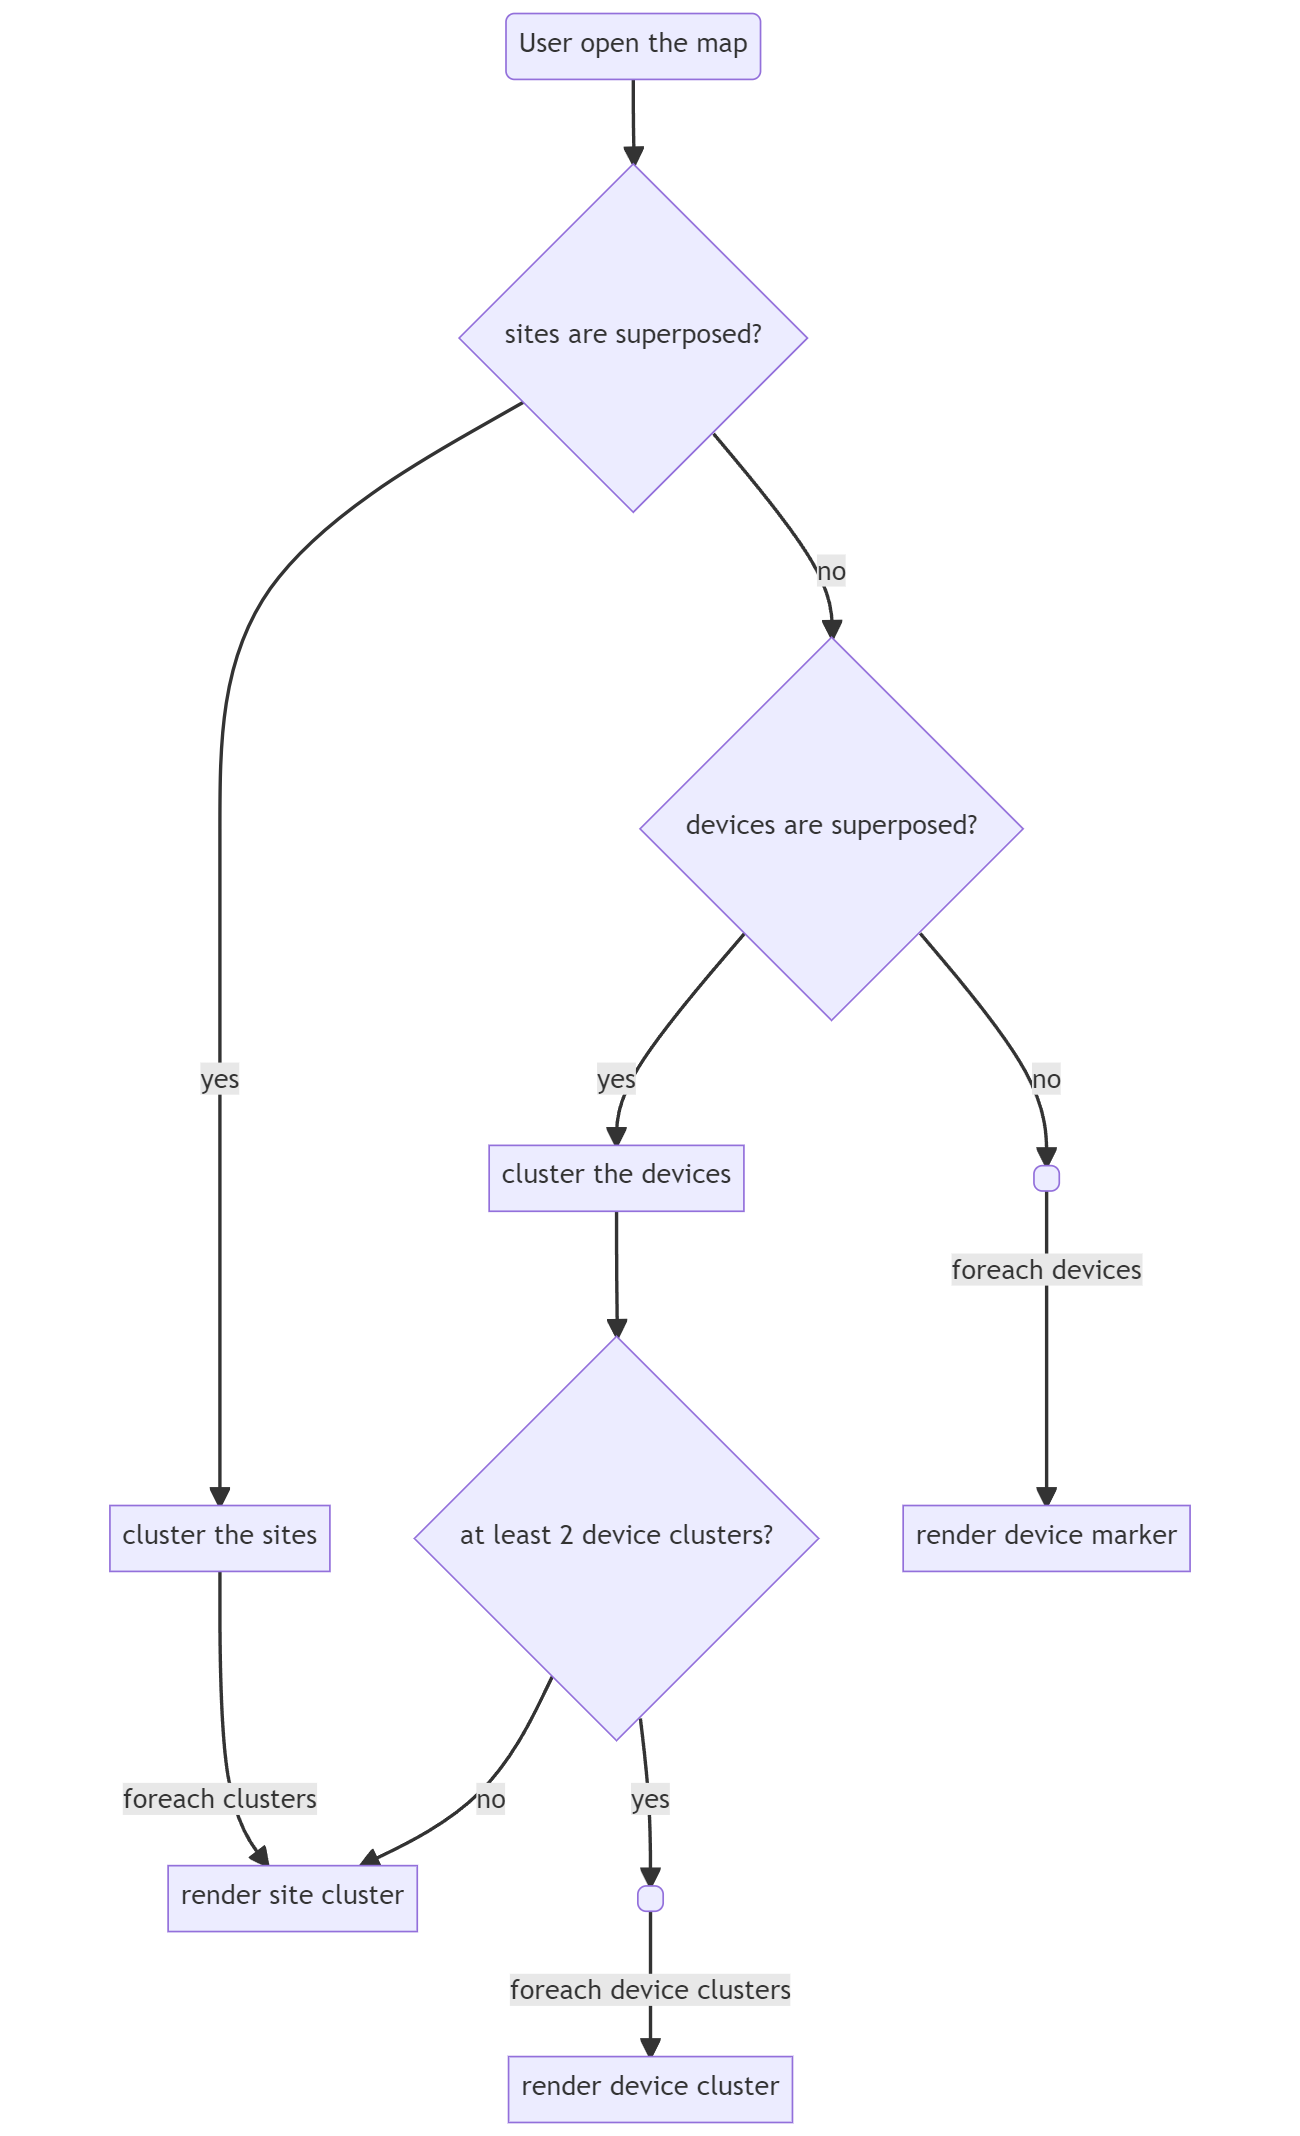
\includegraphics[width=10cm]{map_clustering_flow}
  \caption{Flow-Diagram-Darstellung des zweistufigen Clusterings von \textit{Sites} und Sensoren auf einer interaktiven Karte (Englisch)}
  \label{fig:map_clustering_flow}
\end{figure}

\subsection{Darstellung der Cluster und Marker}

Die aktuelle Karte besteht aus acht verschiedenen Markierungen, die die verschiedenen Arten und den Status der Geräte anzeigen:

\begin{figure}[H]
  \centering
  
\includegraphics[width=10cm]{devices_markers}
  \caption{Marker in Form einer Reißzwecke, die den Standort eines Geräts anzeigen}
  \label{fig:devices_markers}
\end{figure}

Jeweils von links nach rechts stellen sie dar:

\begin{enumerate}
  \item Sensor, der ein Feuer erkennt
  \item Sensor, der offline ist
  \item Sensor mit niedrigem Batteriestand
  \item Sensor, der seine letzte Nachricht vor mehr als 12 Stunden gesendet hat
  \item Sensor, der seine letzte Nachricht vor mehr als 6 Stunden gesendet hat
  \item Aktiver Sensor
  \item Mesh-Gateway
  \item Border-Gateway
\end{enumerate}

Sechs verschiedene Markierungen zu haben, um denselben Gerätetyp anzuzeigen, ist viel zu viel und macht die Verwendung verschiedener Farben weniger relevant.
Es wird empfohlen, eine Palette von maximal fünf Farben zu verwenden \cite{likeChameleon}, damit der Nutzer sie einfach unterscheiden und sich ihre Bedeutung merken kann.
So müssen nur vier Farben verwendet werden, um die verschiedenen Zustände eines Sensors darzustellen.
Dies wird erreicht, indem die Marker 3, 4 und 5 der vorherigen  Liste zu einem einzigen Marker mit der gleichen gelben Farbe wie Marker 5 kombiniert werden.
Dies ist darauf zurückzuführen, dass der Grundstatus hauptsächlich durch eine schlechte Sonneneinstrahlung auf die Solarpaneele oder eine schlechte Abdeckung der LoRa-Verbindung verursacht wurde.
Diese beiden Probleme können direkt vom Kunden behoben werden, indem er einfach einen Sensor neu ausrichtet oder ein Verbindungsrelais hinzufügt.
So wird der neue Status eines Sensors die \textit{Notwendigkeit einer Wartung} anzeigen.\\

Die Karte zeigt nun genau die verschiedenen Geräte eines, aber auch die Position der Cluster von Geräten und \textit{Sites} sowie die Lokalisierung eines einzelnen \textit{Site} müssen dargestellt werden.
In den meisten interaktiven Karten sind Cluster an einem runden Icon zu erkennen, das die Anzahl der enthaltenen Elemente anzeigt und von einem ähnlich gefärbten, aber weniger undurchsichtigen Halo umgeben ist.

\begin{figure}[H]
  \centering
  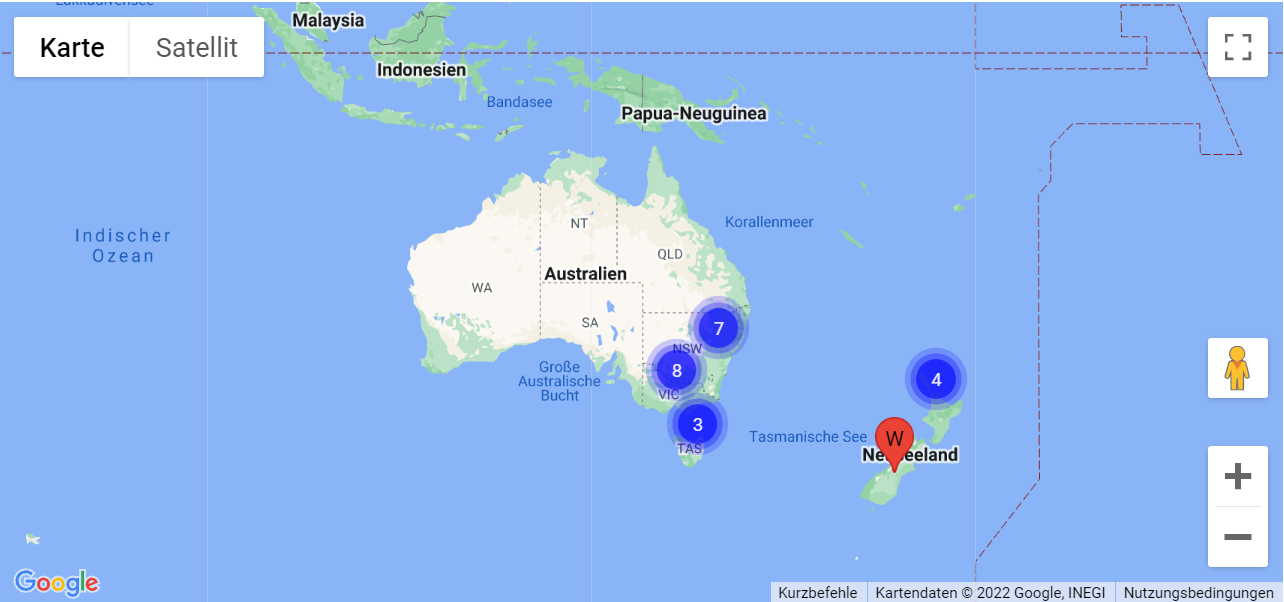
\includegraphics[width=14cm]{google_maps_clusters}
  \caption{Design der Cluster standardmäßig vorhanden auf dem Produkt Google Maps}
  \label{fig:google_maps_clusters}
\end{figure}

Um den Karten von Dryad eine persönliche Note zu verleihen, werden die verschiedenen Cluster durch ein Sechseck dargestellt, das an das Logo des Startups erinnert:

\begin{figure}[H]
  \centering
  
\includegraphics[width=8cm]{clusters_markers}
  \caption{Prototyping von Clustermarkern, die in Version 2 der interaktiven Karten verwendet werden}
  \label{fig:clusters_markers}
\end{figure}

Diese Marker repräsentieren jeweils von links nach rechts:

\begin{enumerate}
  \item Cluster von \textit{Sites}, der einen \textit{Site} enthält, der ein Feuer detektiert
  \item Cluster von \textit{Sites}, der einen \textit{Site} mit einem Offline-Sensor enthält
  \item Cluster von \textit{Sites}, der einen \textit{Site} mit einem wartungsbedürftigen Sensor enthält
  \item Cluster von Standorten
  \item Cluster von Sensoren. Diese Art von Cluster hat die gleichen Farbvariationen wie die \textit{Sites}-Cluster
\end{enumerate}

Die verschiedenen Marker, die Sie verwenden können, sind nun festgelegt.
Um ihr Aussehen entsprechend ihrer Priorität zu verstärken, können Sie die Größe der einzelnen Marker beeinflussen.
So wurde eine Prioritätsskala der Marker und ihrer relativen Größe wie folgt erstellt:

\begin{table}[H]
  \begin{tabular}{p{0.6\linewidth} |p{0.2\linewidth}|p{0.2\linewidth}}
    Markern                                                & Priorität (1: niedrig; 6: hoch) & Relative Größe \\ \hline\hline

    Cluster eines \textit{Site}                            & \textbf{6}                      & x1.11          \\\hline
    Marker einer \textit{Site}                             & \textbf{5}                      & x1             \\\hline
    Cluster von Sensoren in Feuer, offline oder in Wartung & \textbf{4}                      & x0.89          \\\hline
    Cluster von Sensoren                                   & \textbf{2}                      & x0.73          \\\hline
    Marker für einen brennenden Sensor                     & \textbf{4}                      & x0.89          \\\hline
    Marker eines Offline-Sensors                           & \textbf{3}                      & x0.78          \\\hline
    Marker eines Sensors in Wartung                        & \textbf{2}                      & x0.73          \\\hline
    Marker eines Sensors                                   & \textbf{1}                      & x0.55          \\\hline
    Marker eines Border-Gateways                           & \textbf{3}                      & x0.78
  \end{tabular}
  \caption{Festlegung der Prioritäten und Größen der Marker}
\end{table}

Diese relativen Größen bleiben subtil, aber dennoch stark genug, um vom menschlichen Auge erkannt zu werden, wodurch die verschiedenen Prioritäten angezeigt werden können.
Beachten Sie auch, dass eine Markierung mit einer höheren Priorität vor einer Markierung mit einer niedrigeren Priorität angezeigt wird.

\begin{figure}[H]
  \centering
  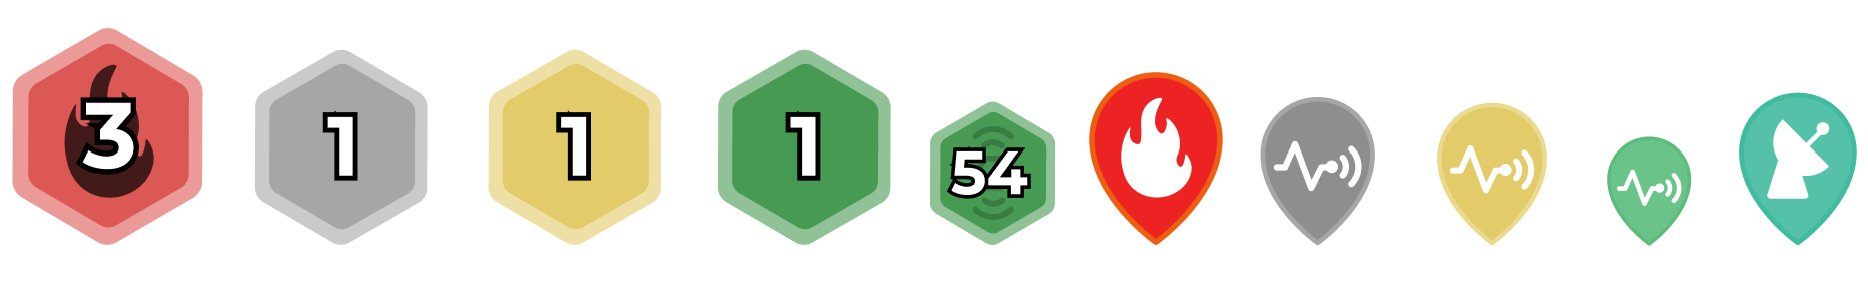
\includegraphics[width=\textwidth]{map_markers_size}
  \caption{Markern mit ihrer relativen Größe auf der Karte}
  \label{fig:map_markers_size}
\end{figure}


\subsection{Hilfe beim Lesen der Karte}

Die Anzeige verschiedener Markierungen ermöglicht bereits eine gute Erkundung eines Ortes und seiner verschiedenen Sensoren.
Es muss noch sichergestellt werden, dass weitere nützliche Hinweise vorhanden sind, die dem Nutzer das Lesen der Karte erleichtern.
Dies gilt insbesondere für die Darstellung eines Standorts, eines Feuers und auch für Informationen, die in einem Cluster zusammengefasst sind.

Ein Standort wird in Form eines Clustermarkers dargestellt.
Um das Auffinden eines bestimmten \textit{Site} auf einer Karte zu erleichtern, wird der Name des \textit{Site} in einem Popup über dem Marker angezeigt, wenn sich die Maus des Nutzers über dem Marker befindet.

\begin{figure}[H]
  \centering
  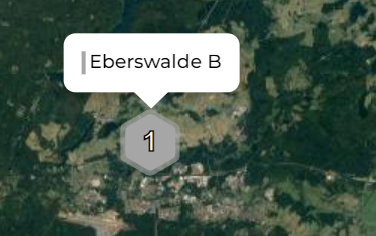
\includegraphics[width=5cm]{map_site_name_window}
  \caption{Popup, das den Namen der \textit{Site} angibt, die von der Maus des Nutzers angehoben wird}
  \label{fig:map_site_name_window}
\end{figure}

Wenn die verschiedenen Geräte einer \textit{Site} in mindestens zwei verschiedenen Clustern angezeigt werden können, verschwindet die Markierung der \textit{Site} und es werden nur noch die Cluster der Geräte angezeigt.
Es ist notwendig, dem Nutzer klar anzuzeigen, zu welcher \textit{Site} diese Geräte gehören.
Um dies zu erreichen, werden die Apparate in einen Bereich eingebettet, der je nach Status der \textit{Site} farbig ist.
Das Popup mit dem Namen der \textit{Site} wird auch sichtbar, wenn der Nutzer mit der Maus über diesen Bereich fährt.

\begin{figure}[H]
  \centering
  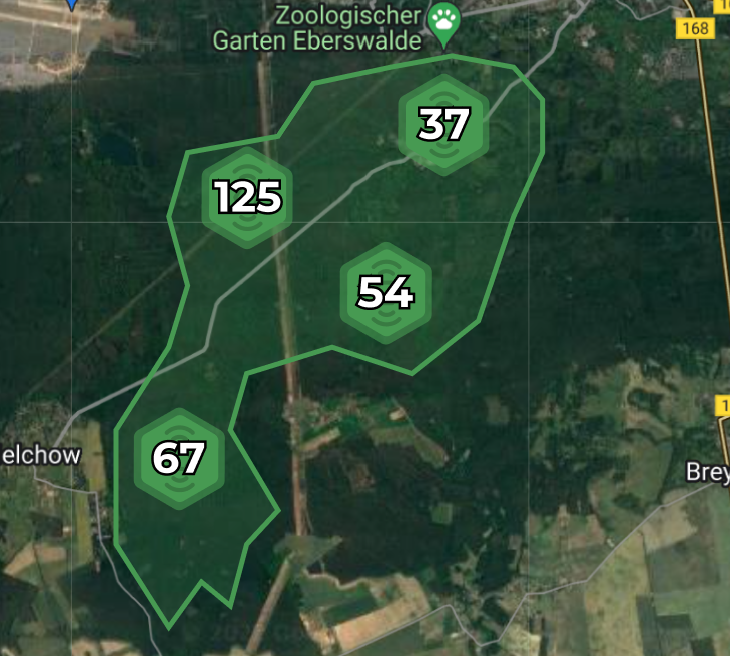
\includegraphics[width=4cm]{map_site_with_zone}
  \caption{Darstellung eines \textit{Site} mit seinem Abdeckungsbereich}
  \label{fig:map_site_with_zone}
\end{figure}

Es ist auch wichtig, jetzt zu definieren, was der Status einer \textit{Site} ist.
Jeder Sensor auf einer \textit{Site} hat einen Status, der Feuer, Offline, Wartung oder Default (nichts zu melden) sein kann.
Ein \textit{Site} oder Sensors-cluster kann Sensoren enthalten, die unterschiedliche Status haben.
Es ist daher notwendig, jedem Status eine Priorität zuzuweisen, um dem Nutzer die relevantesten Informationen anzuzeigen.
So ist es z.B. besser, einen Standort auf der Karte als brennend anzuzeigen, als die Tatsache, dass einer der Sensoren, die ihn bilden, offline ist.

\begin{table}[H]
  \begin{tabular}{p{0.3\linewidth}|p{0.4\linewidth}}
    \centering
    Status     & Priorität (1: niedrig; 4: hoch) \\ \hline\hline

    in Brand   & 4                               \\\hline
    offline    & 3                               \\\hline
    in Wartung & 2                               \\\hline
    Standard   & 1
  \end{tabular}
  \caption{Festlegung der Prioritäten der Status von Sensoren, \textit{Sites} und Clustern}
\end{table}

So hat ein \textit{Site} oder ein Cluster von Sensoren oder ein Cluster von \textit{Sites} den Status (und damit konkret die Farbe) des Sensors mit dem stärksten Status.
Auf diese Weise zeigt ein Cluster nicht alle Informationen der Sensoren an, aus denen er besteht.
Um zu vermeiden, dass der Nutzer die Karte vergrößern muss, um den Status der einzelnen Sensoren zu überprüfen, wird beim Überfahren des Clusters mit der Maus ein Popup mit der Statusverteilung der einzelnen Sensoren eingeblendet.
Diese sollte die Namen der nach Status gruppierten Sensoren sowie einen Balken mit der Verteilung dieser Status anzeigen.

\begin{figure}[H]
  \centering
  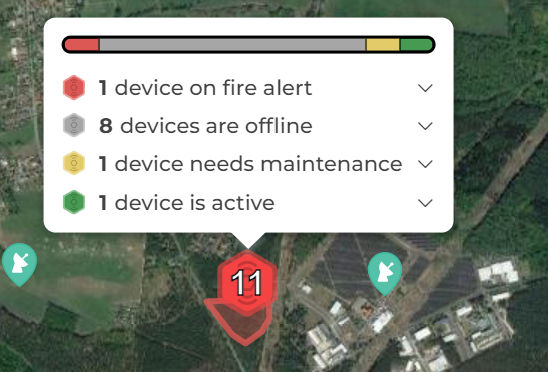
\includegraphics[width=5cm]{map_sensors_window_collapsed}
  \caption{Detailansicht der Sensoren, aus denen ein Cluster besteht}
  \label{fig:map_sensors_window_collapsed}
\end{figure}
\begin{figure}[H]
  \centering
  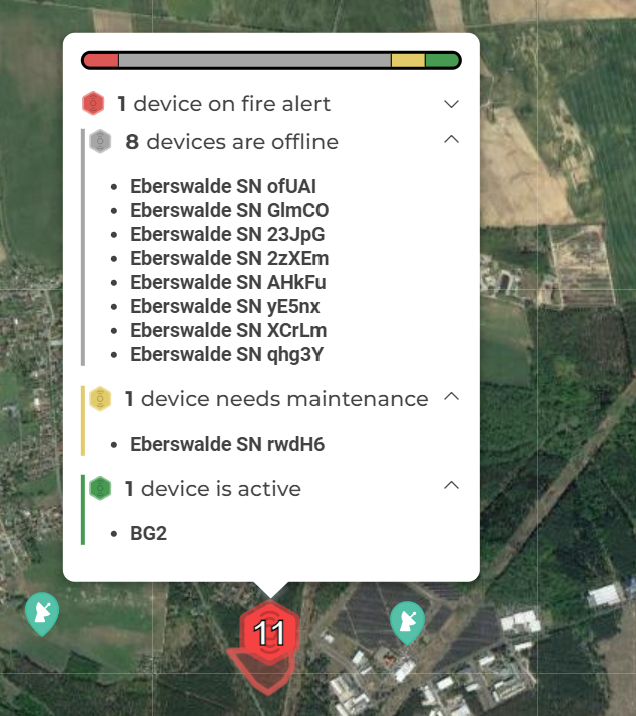
\includegraphics[width=5cm]{map_sensors_window}
  \caption{Detailansicht der Sensoren mit erweiterter Ansicht, die einen Cluster bilden}
  \label{fig:map_sensors_window}
\end{figure}
\begin{figure}[H]
  \centering
  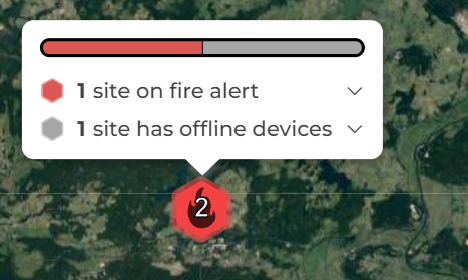
\includegraphics[width=5cm]{map_sites_window}
  \caption{Details zu den \textit{Sites}, aus denen ein Cluster besteht}
  \label{fig:map_sites_window}
\end{figure}

Der stärkste Status ist das Vorhandensein eines Feuers.
Um seine Sichtbarkeit und Erkennung zu verstärken, wird ein Marker eines Sensors mit dem Status \textit{in Feuer} eine Bounce-Animation haben.
